
\documentclass[a4paper]{article}
\usepackage[margin=2cm]{geometry}

\usepackage[utf8]{inputenc}
% \usepackage[polish]{babel}

\usepackage{color, colortbl}
\usepackage[dvipsnames]{xcolor}
\usepackage[section]{placeins}
\usepackage{listings}
\usepackage{graphicx}
\usepackage{cite}
\usepackage{setspace}
\usepackage{mathtools}
\usepackage{natbib}
\usepackage{amsmath}
\usepackage{float}
% \floatstyle{boxed}
% \restylefloat{figure}
\lstset{literate=%
{ą}{{\k{a}}}1
{ć}{{\'c}}1
{ę}{{\k{e}}}1
{ł}{{\l{}}}1
{ń}{{\'n}}1
{ó}{{\'o}}1
{ś}{{\'s}}1
{ż}{{\.z}}1
{ź}{{\'z}}1
{Ą}{{\k{A}}}1
{Ć}{{\'C}}1
{Ę}{{\k{E}}}1
{Ł}{{\L{}}}1
{Ń}{{\'N}}1
{Ó}{{\'O}}1
{Ś}{{\'S}}1
{Ż}{{\.Z}}1
{Ź}{{\'Z}}1,
language=c++,
keywordstyle=\color{gray},
commentstyle=\color{lightgray},
stringstyle=\color{lightgray},
numbers=left,
frame=TBlr,
breaklines=true,
tabsize=2,
numberstyle=\tiny,
basicstyle=\footnotesize \ttfamily
}

\renewcommand\thesection{\arabic{section}.}
\renewcommand\thesubsection{\thesection\arabic{subsection}.}
\renewcommand\thesubsubsection{\thesubsection\arabic{subsubsection}.}
\renewcommand\theparagraph{\thesubsubsection\arabic{paragraph}.}
\renewcommand\thesubparagraph{\theparagraph\arabic{subparagraph}.}

\title{Softcomputing \\ Genetic Algorithms for maxima search of multimodal functions - Report}
\author{\textbf{Krystian Horecki} 181079 \\ 
	\textbf{Antoni Buszta} 181013 \\
	Wroclaw University of Technology}
\date{17.01.2014 r.}

\begin{document}

\maketitle
\newpage
\tableofcontents
\onehalfspace

\section{Project description}
\subsection{Project goals} 
The goal of the project was to create genetic algorithm which will give possibility to find more than one local extremums of the function in case of multi modal functions. 
The main problem in this case is to find version of the algorithm which unlike normal genetic algorithm is able to find more than one result. There exists mechanisms which 
provide such functionality and some of them were used and will be described later in this paper.
Partially the goal was also to check how used genetic algorithm parameters affects results of the computations especially in case of multi modal functions and multi modal optimization process.
\subsection{Used technologies}
To develop solution Python programming language was used with additional library called DEAP\cite{deap} which allows creation of genetic algorithms.
All charts included in this paper were generated with Python library called pyGal\cite{pyGal}. 
\subsection{Examined function}
To determine utility of created solution and test quality of algorithm there was used the Shekel miltimodal function. 
Sheckel function is very useful for this kind of tests because it allows to have the number of maxima is given by the length of any of the 
arguments $\mathcal{A}$ or $\mathbf{C}$, $\mathcal{A}$ is a matrix of size M $\times$ N , where M is the number of maxima and N the number 
of dimensions and c is a M $\times$ 1 vector. The matrix $\mathcal{A}$ can be seen as the position of the maxima and the vector $\mathbf{C}$, the width 
of the maxima. Function equation look as follows: \\
\begin{center}
$f_\text{Shekel}(\mathbf{x}) = \sum_{i = 1}^{M} \frac{1}{c_{i} + \sum_{j = 1}^{N} (x_{j} - a_{ij})^2 }$
\\
\end{center}
To check correctness of algorithm following matrix $\mathcal{A}$ was used: \\
\begin{center}
$\mathcal{A}$ = $
\begin{bmatrix} 0.5 & 0.5 \\ & 0.25 & 0.25 \\ & 0.25 & 0.75 \\ & 
            0.75 & 0.25 \\ & 0.75 & 0.75 \\ & 0.35 & 0.35 \\ &
            1.0 & 1.3 \\ & 1.4 & 0.2 \\ & 0.34 & 1.7 \\ &
            1.5 & 1.3 \\ & 1.1 & 0.9 \\ & 0.9 & 1.7
\end{bmatrix}$ and $\mathbf{C} = 
\begin{bmatrix} 0.002 \\ 0.005 \\ 0.004 \\
            0.003 \\ 0.002 \\ 0.001 \\
            0.002 \\ 0.0023 \\ 0.0035 \\
            0.005 \\ 0.0055 \\ 0.0022 
\end{bmatrix}$, thus defining 12 maximums in $\mathbf{R}^2$. 
\end{center}

Function presented in above equation with given input can be also represented in graphical way which was presented on Figure \ref{sheckel}.

\begin{figure}[h!]
	\centering
	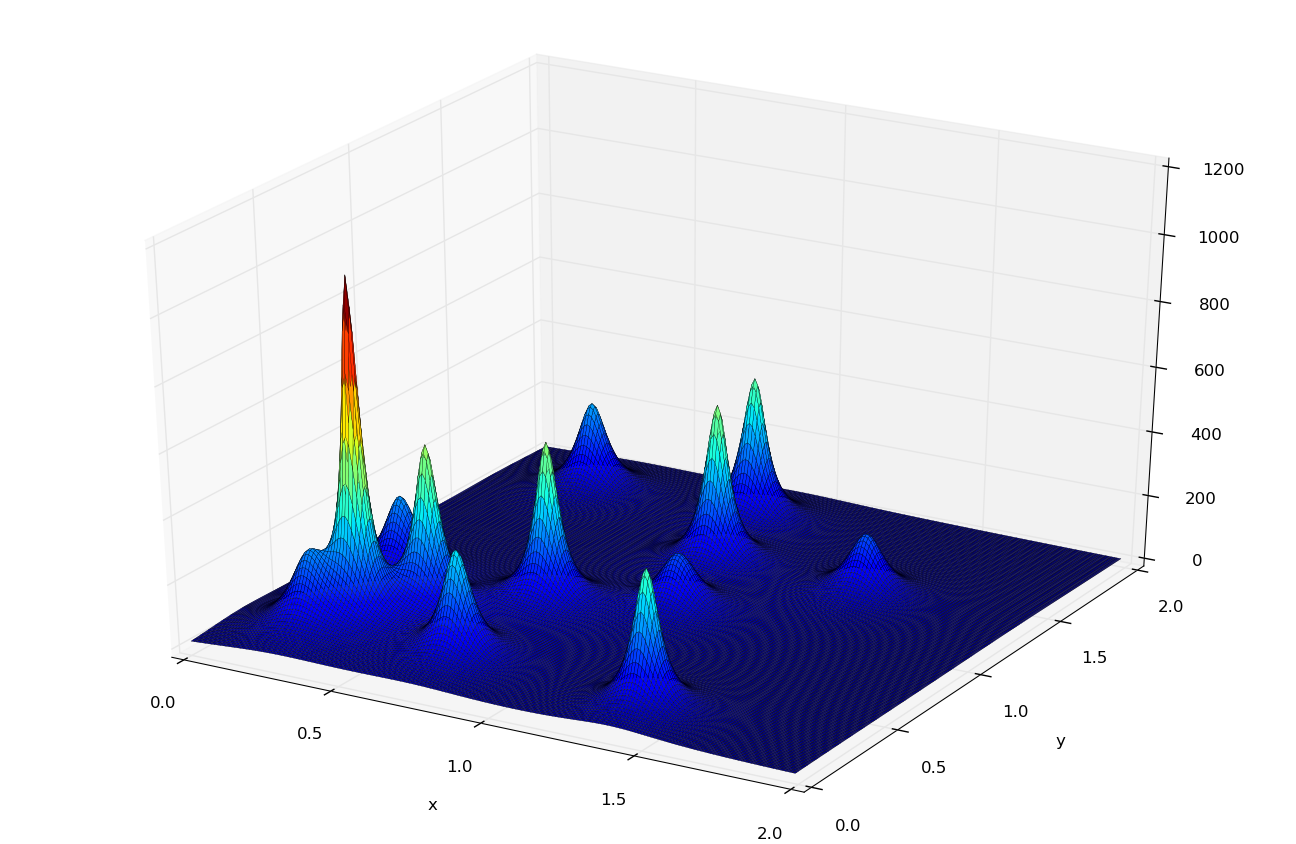
\includegraphics[scale=0.5,keepaspectratio=true]{used_function.png}	
	\caption{Chart of Scheckel function with used A and C input data.}
	\label{sheckel}
\end{figure}
The reson that this kind of function with those parameters was used was to have benchmark which will contain many extremums with different values are scattered in $\mathbf{R}^2$.
\section{Genetic algorithm}
\subsection{Description}
To be able to maintain more than one stable solution and find more than one local extremum it was required to develop modified genetic algorithm. 
Genetic algorithm was develop with niching\cite{niching1,niching2} mechanism which allows to maintain subpopulations of individuals in many niches which gave more than one best solution. 


\subsection{Data representation}
To represent individuals in population a vector with two float values was used. This vector represents point in $\mathbf{R}^2$ and define one individual. As a population the vector of individuals is 
used with length according to population size. Population is generated by creation of random coordinates values for each individual which are within given area of examined space, this action is 
repeated to create as many individuals as it is required. Whole population is later divided into number of subpopulations by choosing and taking random individuals.
\subsection{Niching method}
We used niching mechanism using fitness sharing method which simulate situation when in one niche is only limited number of resources which can be used by individuals. 
Individuals which are occupying the same niche have to share the resources and in case of having too less of them individuals are moving to another niche instead of 
focusing in only one point. To create genetic algorithm with niching it is necessary to define sharing radius $\phi_{share}$ which defines niche size.
The sharing function is defined as:
\[ sh(d_{ij}) = \left
\{\begin{array}{l l}
    1 - (\frac{d_{ij}}{\phi_{share}})^\alpha, & \quad \text{if $d_{ij} < \phi_{share}$}\\
    0, & \quad \text{otherwise}
  \end{array} \right.\]
To calculate $\phi_{share}$ the following equation was used: \\
\[\phi_{share} = \frac{\sqrt{2*|range_{max}-range_{min}|}}{radius factor}\],
where radius factor is parameter given by user.
To calculate shared fitness value equation is defined as:\\
\[f_{share}(i) = \frac{f_{raw}(i)}{\sum_{i=1}^{\pi}sh(d_{ij})}\], \\
where $\pi$ is the representatives vector size. 
Representatives which are used to calculate fitness value are taken from every other subpopulation than currently examined individual and each of them is the best individual from its subpopulation.

\subsection{Mutation method}
Mutation is performed by adding random mutation$\Delta$ value to x and y coordinate. Value of mutation$\Delta$ for each coordinate is calculated with equation defined as
\[mutation\Delta = random(-80, 80)*(range_{max}-range_{min})*0.0001\]

Later value of new coordinates for given individual is calculated with equation defined as\\

\[ individual[x] = \left
\{\begin{array}{l l}
    individual[x] + mutation\Delta, & \quad \text{if individual[x] + mutation$\Delta <= range_{max}$ or $>= range_{min}$}\\
    range_{max}, & \quad \text{if individual[x] + mutation$\Delta > range_{max}$}\\
    range_{min}, & \quad \text{if individual[x] + mutation$\Delta < range_{min}$}
  \end{array} \right.\]

\[ individual[y] = \left
\{\begin{array}{l l}
    individual[y] + mutation\Delta, & \quad \text{if individual[y] + mutation$\Delta <= range_{max}$ or $>= range_{min}$}\\
    range_{max}, & \quad \text{if individual[y] + mutation$\Delta > range_{max}$}\\
    range_{min}, & \quad \text{if individual[y] + mutation$\Delta < range_{min}$}
  \end{array} \right.\]

\subsection{Crossing method}
The method of crossing which was used is simply setting y coordinate from first individual to second one and vice versa. This method can be described with equation defined as \\
\[
\begin{array}{l}
individual_{first_{new}}[x] = individual_{first}[x]\\
individual_{first_{new}}[y] = individual_{second}[y]\\
individual_{second_{new}}[x] = individual_{second}[x]\\
individual_{second_{new}}[y] = individual_{first}[y]
\end{array}\]\\
\subsection{Evaluation method}
During the evaluation of given individual 3 values are taken into account and those are:
\begin{itemize}
 \item{value of function in given point,}
 \item{absolute value of derivative of function on X axis in given point,}
 \item{absolute value of derivative of function on Y axis in given point.}
\end{itemize}
Having listed above parameters it is possible to determine how much given individual fit to maximum definition and promote it or not during selection. 
Later those evaluation results are used during selection which is performed by tournament method. During tournament random 3 individuals are used during 
each tournament and later as a result of selection, new population of individuals is returned.
\subsection{Result analysis}
To analyze results gained from the algorithm vectors of real function extremums points and gained results found by algorithm were sorted by value of the function in given point.
Later by iteration through both vectors till end of smaller of them, the absolute error value was calculated by differing real extremum value with calculated one. As a quality 
metric the average error value was used.
\section{Performed tests}
\subsection{Description}
To check the best set of parameters which gives the best results of searching multiple maxima several tests were performed. Following tests were performed:
\begin{itemize}
\item tests of average error value for different number of generations,
\item tests of average error value for different population size,
\item tests of average error value for different subpopulations number,
\item tests of average error value for different crossing probability,
\item tests of average error value for different mutation probability,
\item tests of average error value for different ray distance factor.
\end{itemize}
In case of each testcase the default set of parameters was used with following parameters:
\begin{center}
  \begin{tabular}{ l | c }
    \hline
    Maximum X value & 2.0 \\ \hline
    Maximum Y value & 2.0 \\ \hline
    Minimum Y value & 2.0 \\ \hline
    Minimum Y value & 2.0 \\ \hline
    Population size & 150 \\ \hline
    Subpopulation number & 12 \\ \hline    
    Crossing probability & 0.6 \\ \hline
    Mutation probability & 0.1 \\ \hline
    Ray distance factor & 25 \\ \hline  
    Number of generations & 200 \\
    \hline
  \end{tabular}
\end{center}

To make sure that gained results are accurate test for each parameter value was performed 5 times and average value was taken as a result.
     
\subsection{Number of generations test}
In order to check how average error value changes along with number of generations the testcase was prepared, where number of generations is increased by 5 from 5 to 100.
Figure \ref{generations} presents result of the test. It can be clearly seen that average error is going down with increasing number of generations but in case of values bigger than 
50, there is no significant improvement. This can be caused by limited resolution of mutation$\Delta$ value and function containing maximums in form of high peaks.
\vfill
\begin{figure}[ht]
	\centering
	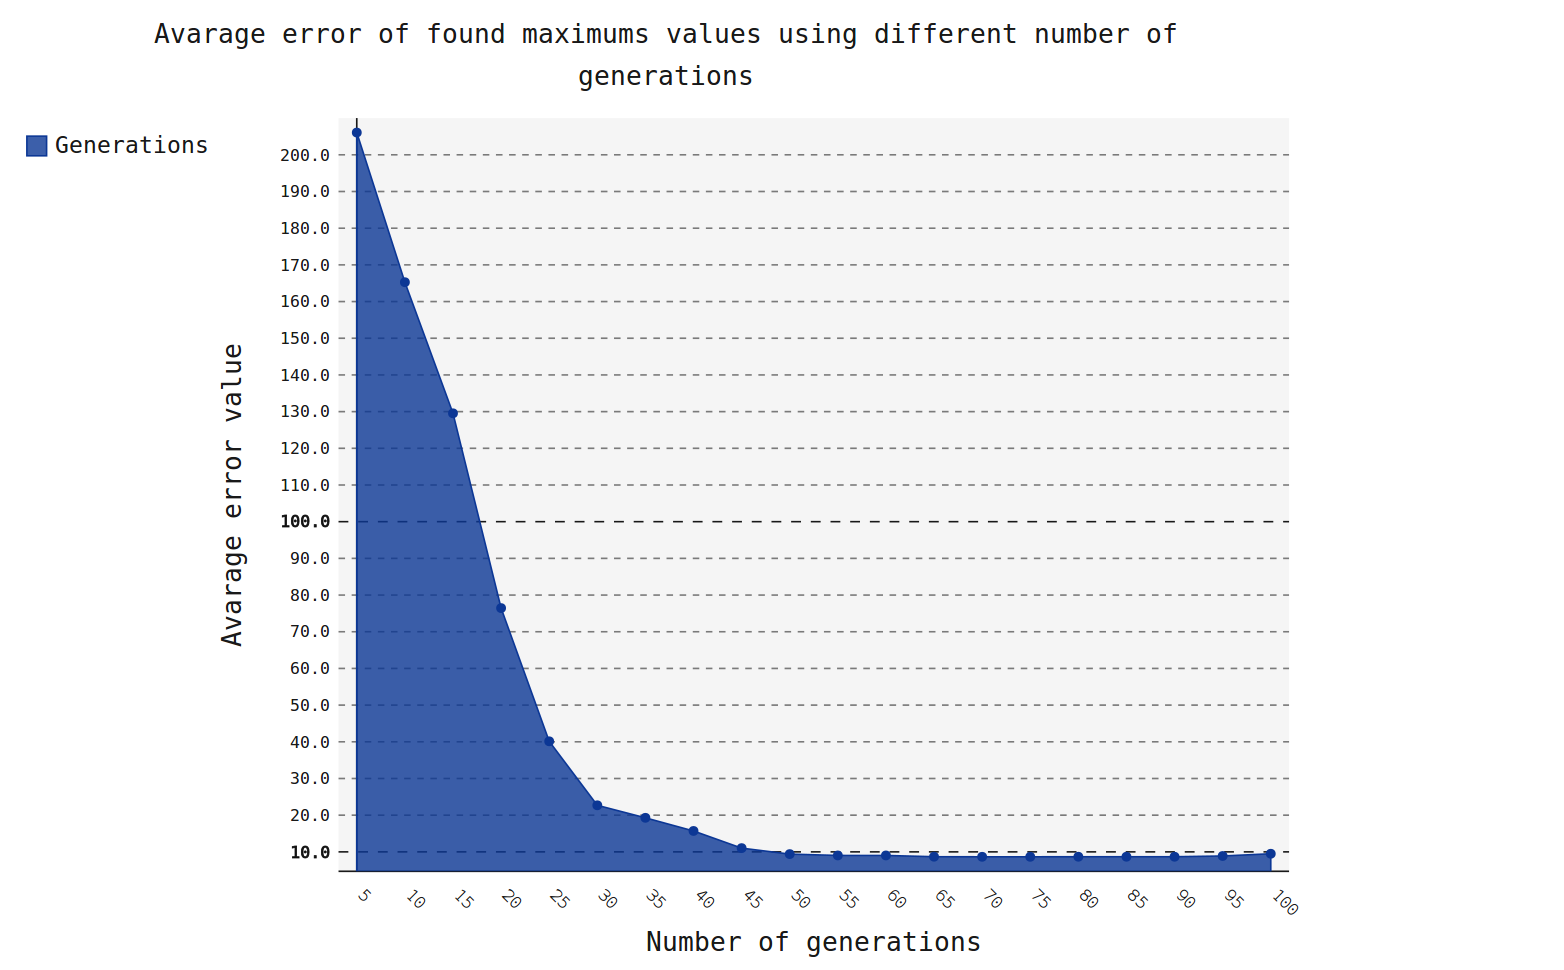
\includegraphics[scale=0.36,keepaspectratio=true]{generations.png}	
	\caption{Results of the algorithm test with different number of generations.}
	\label{generations}
\end{figure}
\vfill
\clearpage


\subsection{Number of individuals in population test}
To check how size of population impact on gained results there was performed test with different population size. Number of individual in population was 
increased by 15 from 15 to 450. As it can be seen on Figure \ref{populations} average error is going down in range of population size between 15 and 75. The best results 
can be obtained using population with size equal to 150. For population size great than 150 average error is increasing which is most likely caused by limited number of resources in each niche.
\vfill
\begin{figure}[ht]
	\centering
	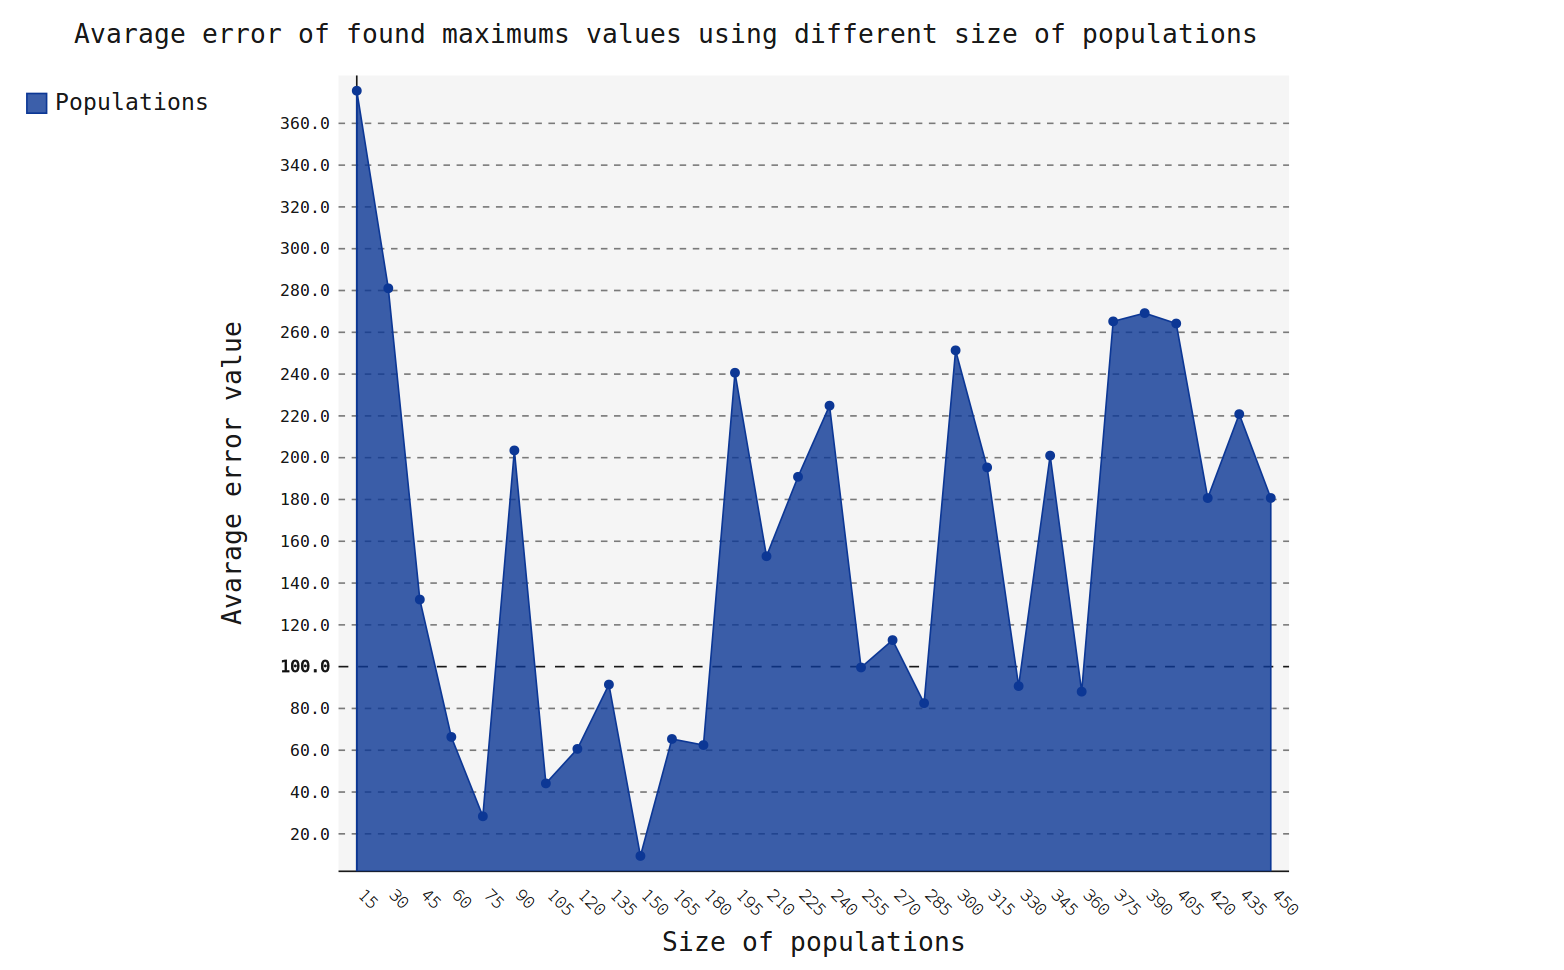
\includegraphics[scale=0.36,keepaspectratio=true]{population.png}	
	\caption{Results of the algorithm test with different sizes of population.}
	\label{populations}
\end{figure}
\vfill
\clearpage


\subsection{Number of subpopulations test}
It is very important to have proper number of subpopulations to get best results so test which was performed used different number of subpopulations. Number of subpopulations was 
increased by 1 from 1 to 40. Results of the test can be seen on Figure \ref{subpopulations}
 and it is clear that in case of 12 local maximas, the best results are gained with 12 subpopulations.
\vfill
\begin{figure}[ht]
	\centering
	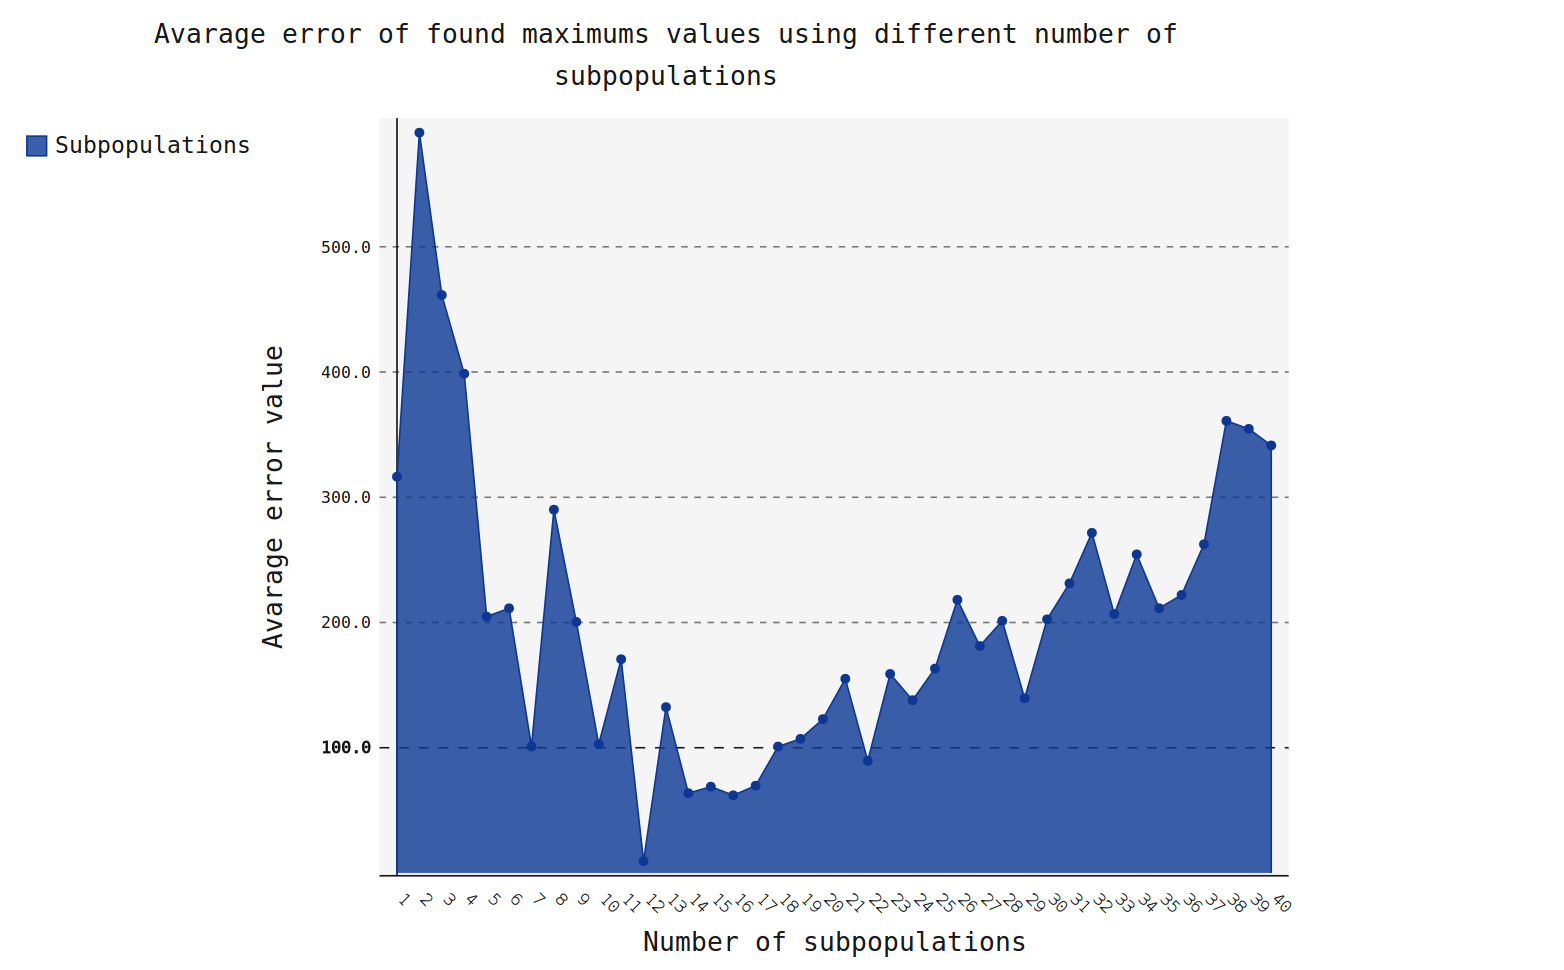
\includegraphics[scale=0.36,keepaspectratio=true]{subpopulation.png}	
	\caption{Results of the algorithm test with different number of subpopulation.}
	\label{subpopulations}
\end{figure}
\vfill
\clearpage

\subsection{Crossing probability test}
To check how crossing probability of two individuals is affecting results, test with changing crossing probability was performed. 
Probability was increased by 0.05 from 0.05 to 1.0. Figure \ref{crossing} presents results of the test which show that best results are reached using probability equal to 0.6.
\vfill
\begin{figure}[ht]
	\centering
	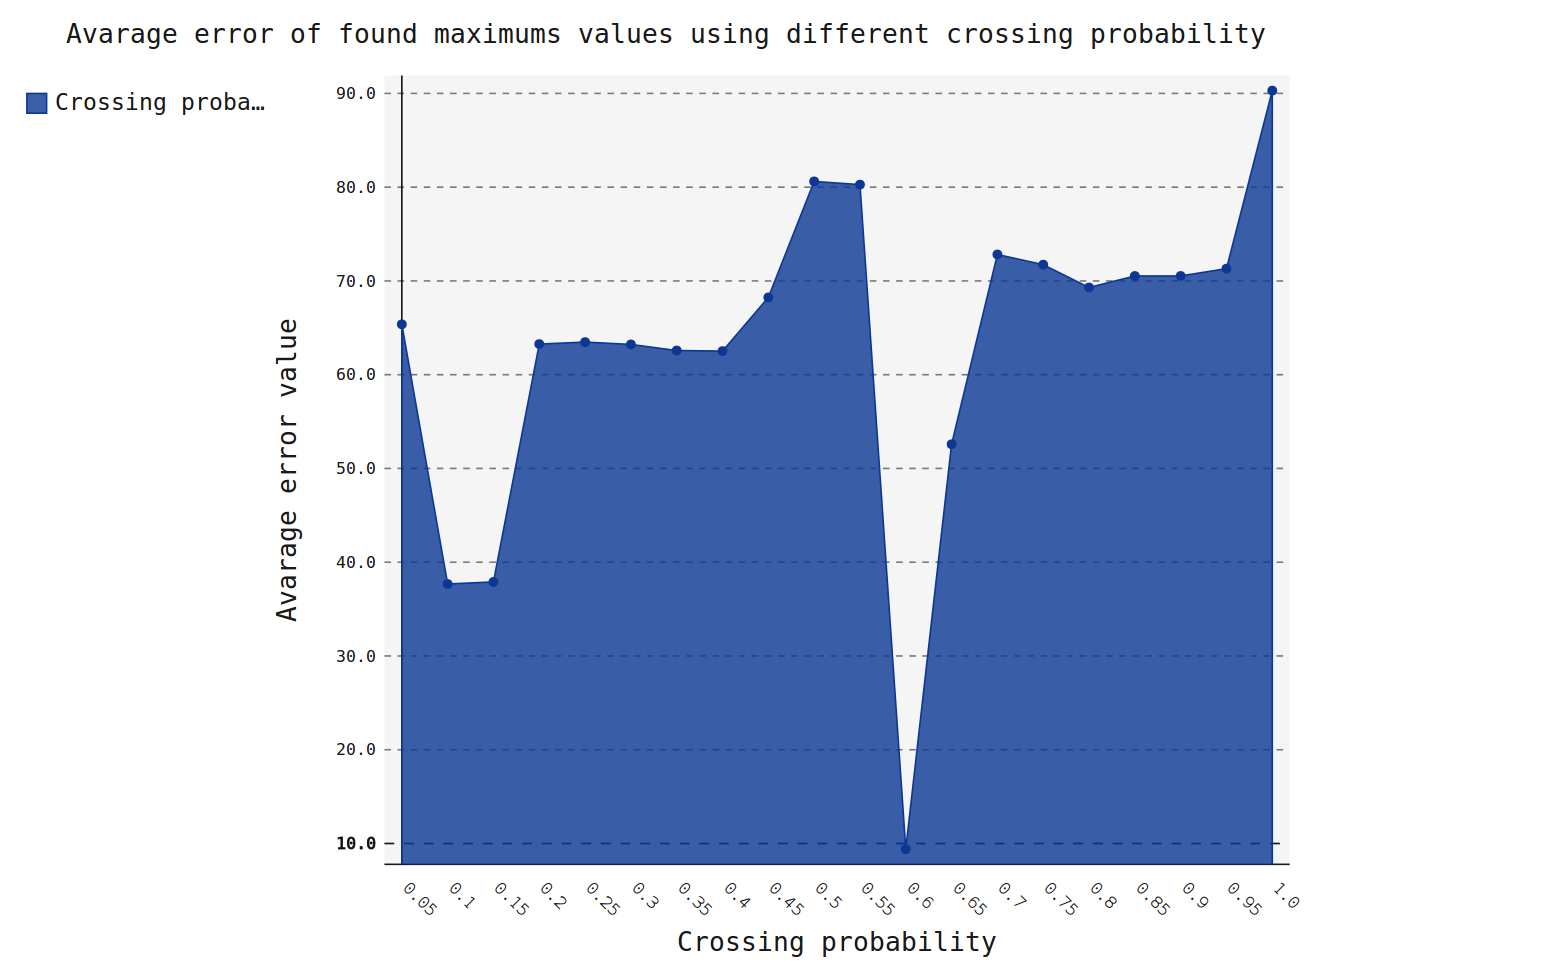
\includegraphics[scale=0.36,keepaspectratio=true]{crossing.png}	
	\caption{Results of the algorithm test with different crossing probabilities.}
	\label{crossing}
\end{figure}
\vfill
\clearpage


\subsection{Mutation probability test}
To check how mutation probability of two individuals is affecting results, test with changing mutation probability was performed. 
Probability was increased by 0.05 from 0.05 to 1.0. Figure \ref{mutation} presents results of the test which show that best results are reached using probability equal to 0.1.
\vfill
\begin{figure}[ht]
	\centering
	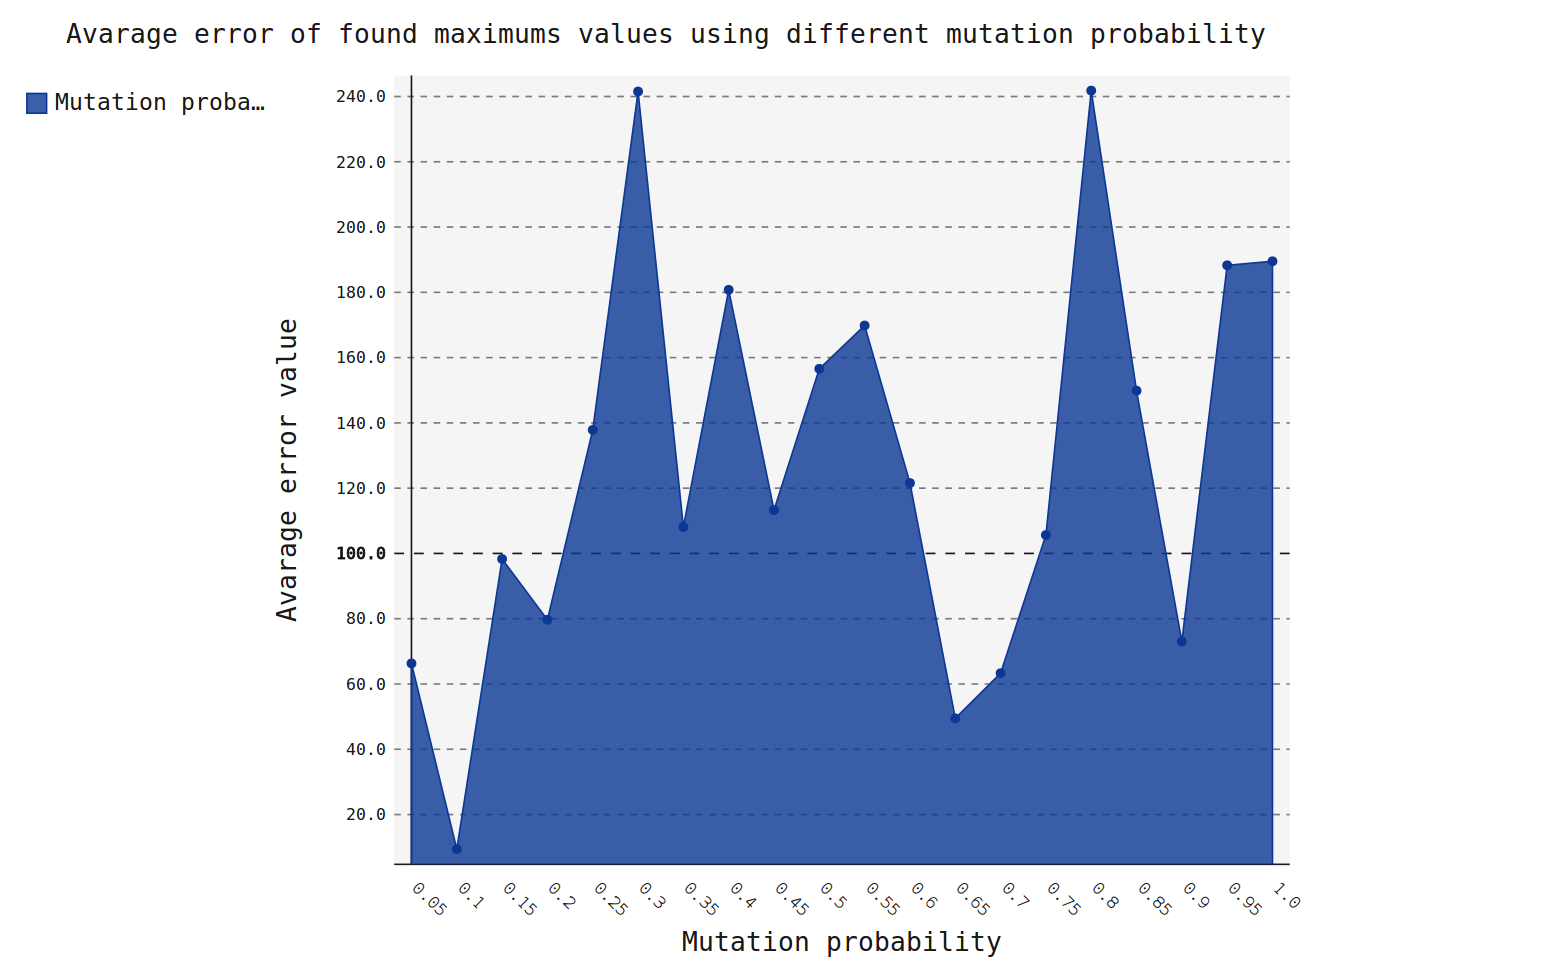
\includegraphics[scale=0.36,keepaspectratio=true]{mutation.png}	
	\caption{Results of the algorithm test with different mutation probabilities.}
	\label{mutation}
\end{figure}
\vfill
\clearpage


\subsection{Ray distance used for niching test}
In case of using niching mechanism it is very important to properly define size of niches to gain best results of computations. 
The ray distance factor which is used to multiply ray of the niche was used as a test parameter and it was checked how it affect work of the algorithm. 
Test checked the value of the average error for different niche ray values. Figure \ref{ray} presents results of the test which shows that error 
is decreasing along with niche ray but there is no significant improvement for values smaller than 0.02.
\vfill
\begin{figure}[ht]
	\centering
	
	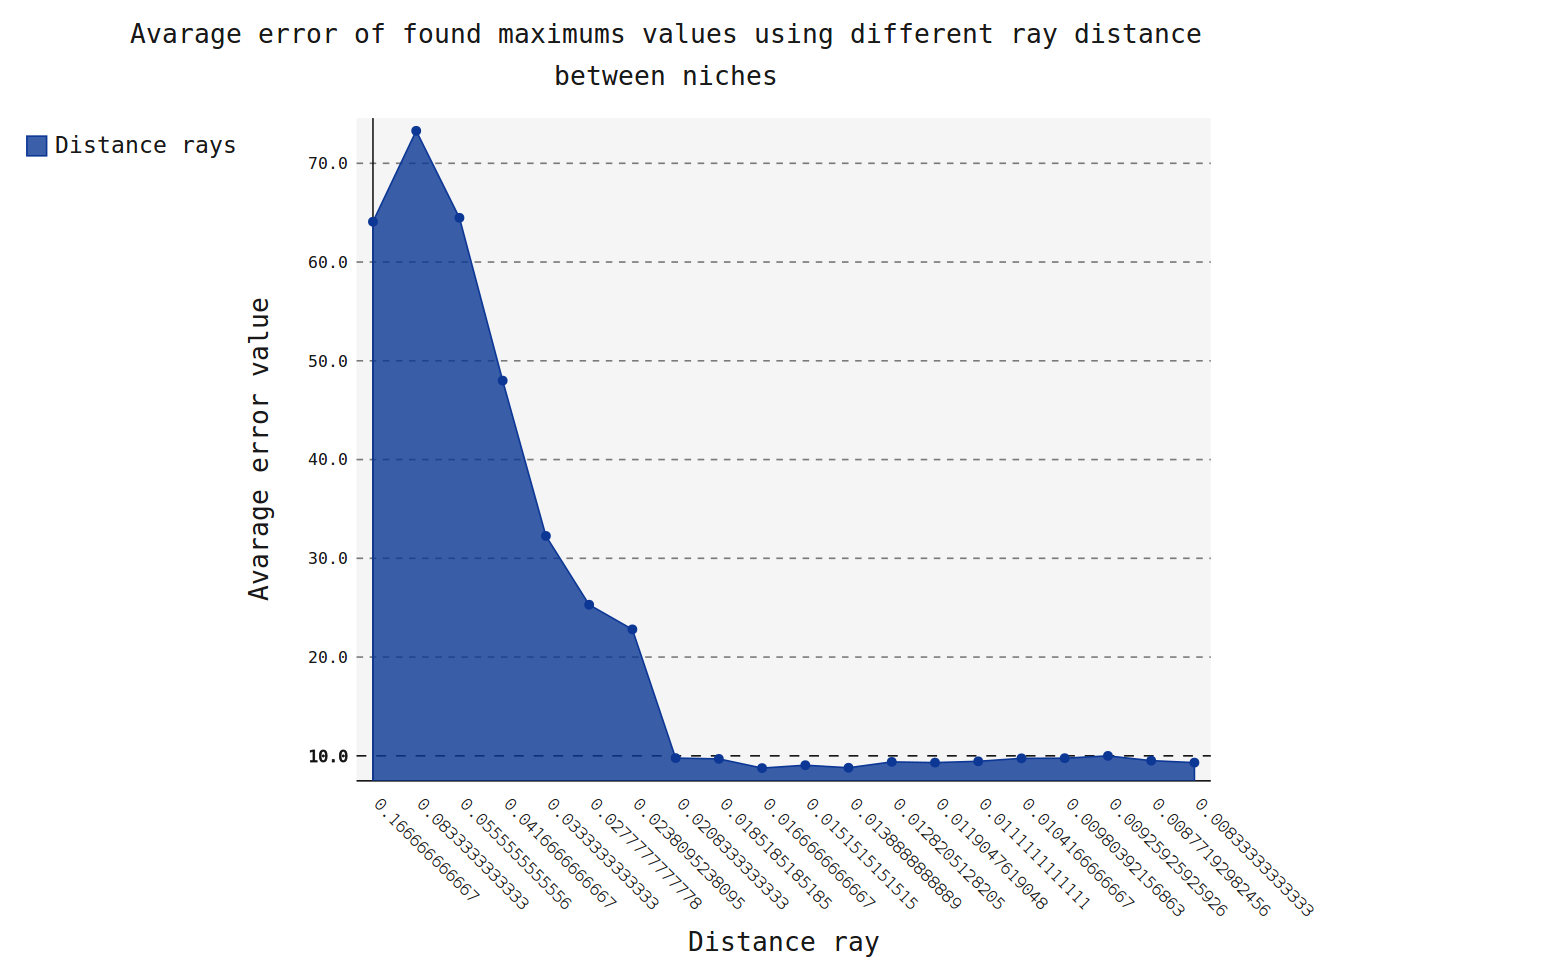
\includegraphics[scale=0.36,keepaspectratio=true]{distance.png}	
	\caption{Results of the algorithm test with different ray distance factor.}
	\label{ray}
	
\end{figure}
\vfill
\clearpage

\section{Final remarks}
Using genetic algorithms with niching mechanism is a very good solution for searching extremums in multi modal functions. Unfortunately the biggest problem on case of this kind 
of algorithm is to properly define input parameters especially distance radius factor and number of subpopulations. Those two parameters depends on type of  the function and number of 
extremums which are searched so it is really hard to define universal values equation. 
\newpage
\listoffigures
\bibliographystyle{plain}
\bibliography{report}

\end{document}
